\documentclass[11pt,a4paper]{article}

% --- Packages ---
\usepackage[utf8]{inputenc}
\usepackage[T1]{fontenc}
\usepackage{lmodern}
\usepackage[margin=1in]{geometry}
\usepackage{amsmath,amssymb,mathtools}
\usepackage{booktabs}
\usepackage{graphicx}
\usepackage{caption}
\usepackage{enumitem}
\usepackage{microtype}
\usepackage{xcolor}
\usepackage[colorlinks=true, linkcolor=blue!70!black, citecolor=blue!70!black, urlcolor=blue!70!black]{hyperref}

% --- Document Metadata ---
\title{\vspace{-1.5cm}
    \large\textbf{Università degli Studi di Cagliari}\\
    \normalsize Faculty of Economic, Legal and Political Sciences\\
    \normalsize Master in Economics, Finance and Data Analysis\\[1.5ex]
    \Large\textbf{Spatial and Regional Economics (Module A)}\\
    \large\textbf{Homework 1: The Rosen--Roback Spatial Equilibrium Model}\\
    \normalsize Academic Year 2026--2027
}

\author{
    \textbf{Team Members:}\\[0.5ex]
    Davide Maiellaro \quad Caterina Congia\\[0.5ex]
    Federica Stella Favalli \quad Lorenzo Piva
}

\date{October 14, 2026}

\begin{document}

\maketitle

\vspace{-0.5cm}
\begin{center}
    \small
    \textbf{Instructor:} Prof. Fabio Cerina \quad$\vert$\quad \textbf{Discussion \& Presentation Date:} October 14, 2026
\end{center}
\vspace{0.2cm}

% --- AI Disclosure (required by the assignment) ---
\noindent\fbox{%
    \parbox{\dimexpr\linewidth-2\fboxsep-2\fboxrule}{%
        \footnotesize
        \textbf{AI Disclosure Statement.} The team used two AI assistants: Google Gemini (first draft of the \LaTeX{} text and debugging of the Matlab block) and Claude by Anthropic (review of the derivations, consistency check of the reported numbers, \LaTeX{} editing). All derivations, numerical results and interpretations were checked by the authors, who re-ran every script reported here.
    }%
}

\vspace{0.5cm}

% =========================================================================
% PART A: THE PUZZLE (MODEL WITHOUT LAND, TOPIC 2)
% =========================================================================
\section*{Part A -- The Puzzle: Model without Land (Topic 2)}

\noindent Throughout, $n = 60$, $\bar L = 10^5$, $\gamma = 0.3$, $K_i = 1$, seed \texttt{rng(7)}. The model and its inversion on data $(L_i, w_i)$ are
\begin{equation}
    w_i = A_i K_i^{\gamma} L_i^{-\gamma}, \qquad U_i = w_i B_i = W
    \quad\Longrightarrow\quad
    \hat A_i = w_i L_i^{\gamma} K_i^{-\gamma}, \qquad \hat B_i = \frac{W}{w_i},
    \label{eq:inversion}
\end{equation}
with $W$ fixed by the normalization $\frac{1}{n}\sum_i \hat B_i = 1$ (function \texttt{rr\_invert}). In logs, $\ln \hat B_i = \ln W - \ln w_i$: recovered amenities are the mirror image of wages.

% -------------------------------------------------------------------------
\subsection*{(a) The population--amenities panel in the original script}

\paragraph{What the script does.} The original data-generating block draws $L_i \sim \text{Uniform}(0,1)$, rescaled so that $\sum_i L_i = \bar L$, and, \emph{independently}, $w_i \sim \text{Uniform}(0.5,\,2)$. It then inverts these data with \eqref{eq:inversion} and plots the four panels of Figure~\ref{fig:a}. The printed OLS slopes are in Table~\ref{tab:a}.

\begin{figure}[htbp]
    \centering
    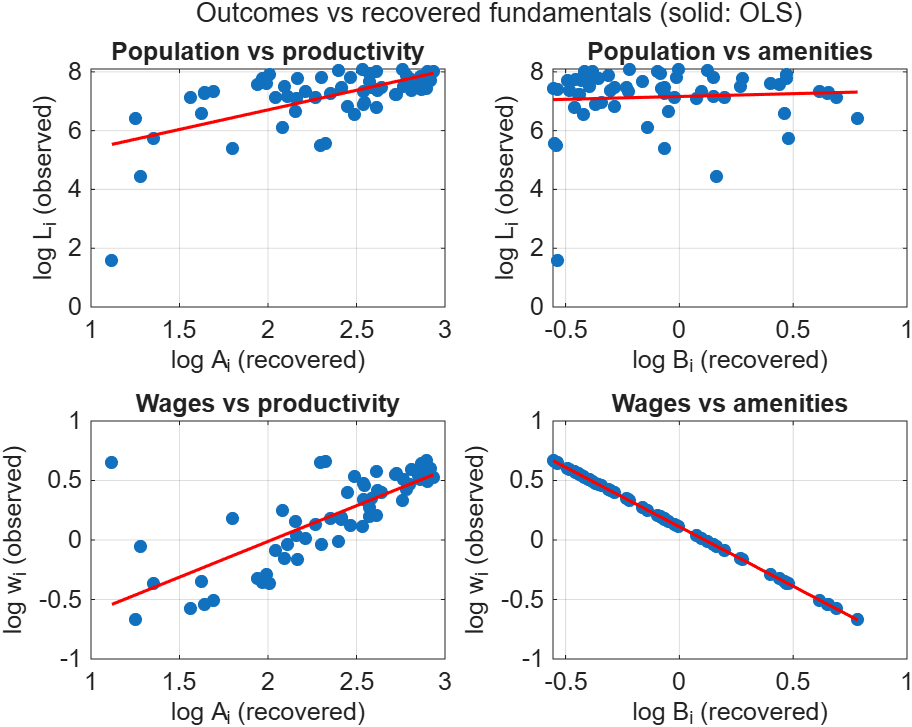
\includegraphics[width=0.75\textwidth]{figures/RR1_hw_scatter_a.png}
    \caption{Original script ($L$ and $w$ drawn independently). Top right: population vs recovered amenities.}
    \label{fig:a}
\end{figure}

\begin{table}[htbp]
    \centering
    \caption{OLS slopes, original data-generating block}
    \label{tab:a}
    \begin{tabular}{llr}
        \toprule
        \textbf{Panel} & \textbf{Regression (logs)} & \textbf{Slope} \\
        \midrule
        Population vs productivity & $\ln L_i$ on $\ln \hat A_i$ & $1.333$ \\
        \textbf{Population vs amenities} & $\ln L_i$ on $\ln \hat B_i$ & $\mathbf{0.192}$ \\
        Wages vs productivity & $\ln w_i$ on $\ln \hat A_i$ & $0.600$ \\
        Wages vs amenities & $\ln w_i$ on $\ln \hat B_i$ & $-1.000$ \\
        \bottomrule
    \end{tabular}
\end{table}

\paragraph{Description of the panel.}
\begin{itemize}[leftmargin=1.5em]
    \item \textbf{Sign:} slightly positive, $\hat\beta_{L,B} = 0.192$.
    \item \textbf{Size:} economically and statistically zero. A 1\% higher recovered amenity is associated with only 0.19\% more population. The correlation is $\operatorname{corr}(\ln L, \ln \hat B) = +0.07$, so $R^2 \approx 0.005$ and the $t$-statistic is $t = r\sqrt{n-2}/\sqrt{1-r^2} \approx 0.5$. The points form a shapeless cloud, even though both variables vary a lot: $\ln L_i$ goes from about 1.6 to 8.1 and $\ln \hat B_i$ from $-0.56$ to $0.78$, so amenities differ by a factor of almost 4.
\end{itemize}

\paragraph{Why this is surprising given $U_i = w_i B_i$.}
People value amenities, since $\partial U_i/\partial B_i = w_i > 0$. Mobility should therefore send them to high-$B$ places. Indeed, in equilibrium (Topic 2, eq.~1) population shares are
\begin{equation}
    \pi_i = \frac{L_i}{\bar L} = \frac{K_i (A_i B_i)^{1/\gamma}}{\sum_j K_j (A_j B_j)^{1/\gamma}},
\end{equation}
increasing in $B_i$. The same holds for the recovered fundamentals: multiplying the two formulas in \eqref{eq:inversion} gives $\hat A_i \hat B_i = W L_i^{\gamma}$ (with $K_i=1$), i.e.
\begin{equation}
    \ln L_i = \tfrac{1}{\gamma}\left(\ln \hat A_i + \ln \hat B_i\right) - \tfrac{1}{\gamma}\ln W .
    \label{eq:LAB}
\end{equation}
For two locations with the same $\hat A$, the one with 1\% higher amenities must be $1/\gamma = 3.33\%$ larger. The evidence shown in Topic~2 points the same way: in Glaeser and Gottlieb (2009), metropolitan population growth rises with mean January temperature, a classic amenity. So we would expect a clearly upward-sloping panel. Instead we get a flat one: this is the anomaly.

\paragraph{Where the flat slope comes from.}
Since $\ln \hat B_i = \ln W - \ln w_i$, the OLS slope of the panel is (derived in part (d))
\begin{equation}
    \hat\beta_{L,B} = -\frac{\widehat{\operatorname{Cov}}(\ln L_i, \ln w_i)}{\widehat{\operatorname{Var}}(\ln w_i)} .
    \label{eq:slope}
\end{equation}
The panel therefore only reflects how $L$ and $w$ co-move in the data. In the original block they are drawn independently, so $\operatorname{Cov}(\ln L, \ln w) = 0$ and the expected slope is zero. The value $0.192$ is pure sampling noise: in this draw $\operatorname{corr}(\ln L, \ln w) = -0.07$. Note that the panel does not hold $\hat A$ fixed. Equation~\eqref{eq:LAB} holds for any data, but in these data a high $\hat B$ (a low wage) also means a low $\hat A$, and the two effects cancel.

% -------------------------------------------------------------------------
\subsection*{(b) Removing the assumption: the urban wage premium}

\paragraph{Which assumption, which fact.}
\begin{itemize}[leftmargin=1.5em]
    \item \textbf{Assumption:} population and wages are drawn independently, which imposes
    \[
        \operatorname{Cov}(\ln L_i, \ln w_i) = 0 .
    \]
    Big and small locations pay, on average, the same wage.
    \item \textbf{Fact:} Topic~1, Fact~4, the urban wage premium. Denser places pay more (Autor, Ely Lecture 2019): log hourly wages rise steadily with log population density across US commuting zones.
\end{itemize}

\paragraph{Choice of $\phi$.}
We replace the independent draw with $\ln w_i = \phi \ln L_i + \text{noise}$. In our model all locations have the same capital ($K_i = 1$) and there is no land, so size and density coincide up to a constant, and the elasticity with respect to density can be used as $\phi$. A back-of-the-envelope reading of the fitted lines in Autor's figure (Topic~1, slide 22) gives the following. Over about three orders of magnitude of density ($\approx 7$ log points), log wages of college workers rise by about 0.5--0.6, an elasticity of about $0.07$--$0.08$. For non-college workers the gradient was similar in 1970 and has since fallen to about $0.02$. We set
\[
    \phi = 0.08, \qquad \sigma_\varepsilon = 0.15 .
\]
The noise term captures wage differences unrelated to size (industry mix, skills). With $\sigma_\varepsilon = 0.15$ the drawn data have $\operatorname{corr}(\ln L, \ln w) \approx 0.5$: a clear but noisy premium, as in the data. As shown in (d), $\sigma_\varepsilon$ only affects the \emph{size} of the slope, never its sign. Any $\phi > 0$ gives the same qualitative answer.

\paragraph{Modified block.}
\begin{verbatim}
ORIGINAL_DGP = false;
phi   = 0.08;            % elasticity of wages to city size (Fact 4, Topic 1)
sig_e = 0.15;            % sd of the wage noise (set to 0 for Part A(d))
L_obs = rand(1, n);                      % same L draw in every case
L_obs = Ltot * L_obs / sum(L_obs);       % rescale so that sum(L) = Ltot
if ORIGINAL_DGP
    w_obs = 0.5 + 1.5 * rand(1, n);      % original: w uniform on [0.5, 2]
else
    lL    = log(L_obs);
    w_obs = exp(phi * (lL - mean(lL)) + sig_e * randn(1, n));
end
\end{verbatim}
In formulas: $\ln w_i = \phi\,(\ln L_i - \overline{\ln L}) + \sigma_\varepsilon \varepsilon_i$, with $\varepsilon_i \sim \mathcal N(0,1)$ independent of $L_i$. Three remarks on the code:
\begin{itemize}[leftmargin=1.5em]
    \item The switch \texttt{ORIGINAL\_DGP = true} reproduces part (a) exactly, so the same file generates every result in this report.
    \item The seed and the $L$ draw come first and are unchanged, so $L_i$ is \emph{identical} to part (a). Only wages change, and the comparison is clean (same vertical axis in Figures~\ref{fig:a} and~\ref{fig:b}).
    \item Subtracting $\overline{\ln L}$ only sets the level of wages (geometric mean around 1, as in the original range $[0.5, 2]$). A constant drops out of every slope.
\end{itemize}

\paragraph{Prediction before running.}
Substituting the new wage equation into the inversion formula $\ln \hat B_i = \ln W - \ln w_i$:
\begin{equation}
    \ln \hat B_i = \text{const} - \phi \ln L_i - \sigma_\varepsilon \varepsilon_i
    \qquad\Longrightarrow\qquad
    \frac{\partial \ln \hat B_i}{\partial \ln L_i} = -\phi = -0.08 < 0 .
    \label{eq:derivB}
\end{equation}
The panel puts $\ln L$ on the vertical axis and $\ln \hat B$ on the horizontal one. The sign of an OLS slope is the sign of the covariance, whichever variable is on the vertical axis. Since $\operatorname{Cov}(\ln L, \ln \hat B) = -\phi \operatorname{Var}(\ln L) < 0$, \textbf{we predict a negative slope}.

We can also predict its size. Using the population moments,
\begin{equation}
    \beta_{L,B} = \frac{-\phi\, v_L}{\phi^2 v_L + \sigma_\varepsilon^2}, \qquad v_L \equiv \operatorname{Var}(\ln L_i) .
    \label{eq:popslope}
\end{equation}
With $L_i$ uniform, $-\ln L_i$ is (up to a constant) exponentially distributed with variance 1, so $v_L \approx 1$ and $\beta_{L,B} \approx -0.08/(0.0064 + 0.0225) \approx -2.8$.

\paragraph{Results.}
\begin{figure}[htbp]
    \centering
    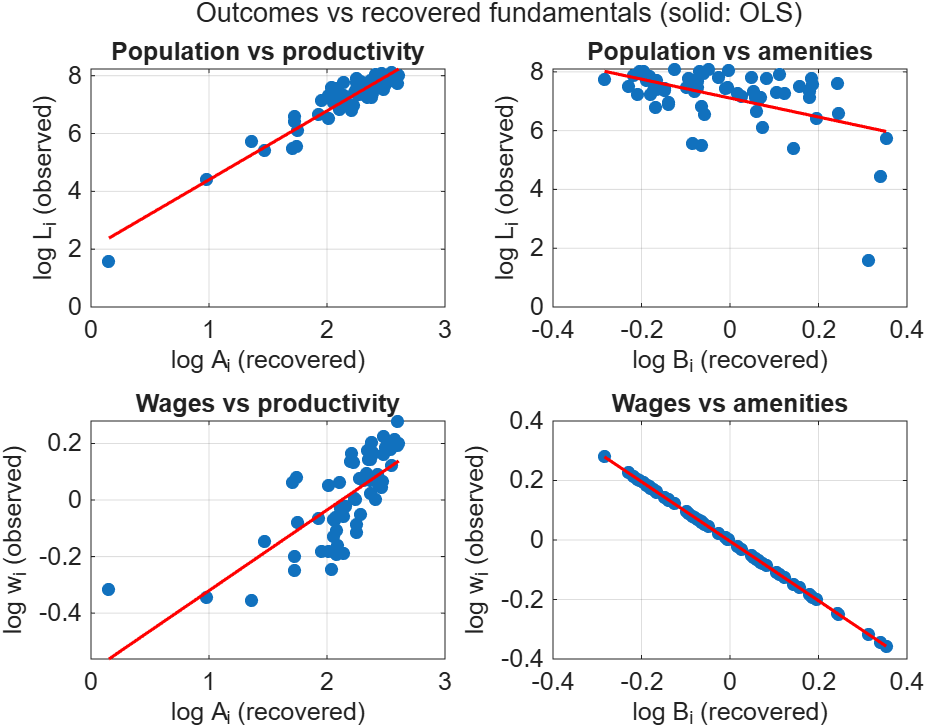
\includegraphics[width=0.75\textwidth]{figures/RR1_hw_scatter_b.png}
    \caption{Modified block: $\ln w_i = \phi \ln L_i + \text{noise}$, $\phi = 0.08$, $\sigma_\varepsilon = 0.15$. Top right: the population--amenities panel is now downward sloping.}
    \label{fig:b}
\end{figure}

\begin{table}[htbp]
    \centering
    \caption{OLS slopes: original vs modified data-generating block}
    \label{tab:b}
    \begin{tabular}{lcc}
        \toprule
        \textbf{Panel} & \textbf{Original (a)} & \textbf{Modified (b)} \\
        \midrule
        Population vs productivity & $1.333$ & $2.382$ \\
        \textbf{Population vs amenities} & $\mathbf{+0.192}$ & $\mathbf{-3.217}$ \\
        Wages vs productivity & $0.600$ & $0.285$ \\
        Wages vs amenities & $-1.000$ & $-1.000$ \\
        \midrule
        $\operatorname{corr}(\ln L, \ln w)$ & $-0.07$ & $+0.49$ \\
        \bottomrule
    \end{tabular}
\end{table}

\noindent The prediction is confirmed (Figure~\ref{fig:b}, Table~\ref{tab:b}). The population--amenities slope turns clearly negative, $\hat\beta_{L,B} = -3.217$, close to the predicted $-2.8$. The gap is sampling variability with $n = 60$, discussed in (d). The wages--amenities panel is still exactly $-1$, because $\ln \hat B_i = \text{const} - \ln w_i$ by construction. The population--productivity panel becomes steeper and tighter, because $\ln \hat A_i = \ln w_i + \gamma \ln L_i$ now increases with $L_i$ through both terms. The wages--productivity slope falls toward $\phi/(\phi+\gamma) \approx 0.21$, because most of the variation in $\hat A$ now comes from $L$ rather than from wage noise (see (d)).

\paragraph{What we conclude about the model without land as a measurement device.}
\begin{enumerate}[leftmargin=1.5em]
    \item \textbf{The inversion always fits, so it cannot flag the problem.} Any $(L,w)$ is rationalized exactly (Topic~2: ``inversion measures, it does not test''). The output is only as good as the model behind it.
    \item \textbf{With a single price, amenities are just the inverse of wages.} Since $\hat B_i \propto 1/w_i$, anything that raises wages in large places, such as the urban wage premium, is read as compensation for bad amenities. Once the data respect Fact~4, the model mechanically concludes that the largest cities are the least pleasant places to live.
    \item \textbf{The missing price is rent.} Topic~1 (Fact~4, cont.) also shows that denser places are more expensive: the elasticity of rents to density is about 0.16. In reality, high wages in big cities largely compensate for high housing costs, not for bad amenities. A model in which the wage is the only price cannot tell an \emph{expensive} place from an \emph{unpleasant} one.
\end{enumerate}
Hence the model without land gives biased amenity measures, which are unlikely to pass an external validation against observable amenities such as climate or coastline (Topic~2, slide 24). Housing must be added, so that amenities are read off rents \emph{and} wages, $B_i \propto r_i^{1-\mu}/w_i$ (Topic~3, Part~B).

% -------------------------------------------------------------------------
\subsection*{(c) Amenity spillovers: total vs exogenous amenities}

Suppose $B_i = b_i L_i^{\eta}$, with $b_i$ exogenous (climate, coast) and $\eta$ the spillover elasticity. If $\eta > 0$, size creates amenities (restaurants, culture, leisure). If $\eta < 0$, size creates disamenities (congestion, pollution) (Topic~1, slide 32).

\paragraph{Panel with recovered total amenities $\hat B_i$: it does not change.}
The mobility condition $w_i B_i = W$ involves only \emph{total} amenities: workers do not care whether $B_i$ comes from nature or from other people. The inversion $\hat B_i = W/w_i$ uses only observed wages, and $\eta$ appears nowhere. Given the same data $(L_i, w_i)$, $\hat B_i$ is numerically identical and the panel is unchanged:
\begin{equation}
    \frac{\partial \ln \hat B_i}{\partial \ln L_i} = -\phi \qquad \text{(same as in (b))}.
\end{equation}

\paragraph{Panel with recovered exogenous amenities $\hat b_i = \hat B_i L_i^{-\eta}$: it changes.}
Taking logs and using \eqref{eq:derivB},
\begin{equation}
    \ln \hat b_i = \ln \hat B_i - \eta \ln L_i = \text{const} - (\phi + \eta)\ln L_i - \sigma_\varepsilon\varepsilon_i
    \qquad\Longrightarrow\qquad
    \frac{\partial \ln \hat b_i}{\partial \ln L_i} = -(\phi + \eta) .
    \label{eq:derivb}
\end{equation}
Each point moves horizontally by $-\eta \ln L_i$, more for larger locations. The sign of the panel is the sign of $-(\phi+\eta)$:
\begin{itemize}[leftmargin=1.5em]
    \item \textbf{Positive spillovers ($\eta > 0$):} $-(\phi+\eta) < -\phi < 0$. Exogenous amenities fall even faster with size. Big cities already get a low total $\hat B$. If their size itself adds amenities, their natural component must be even lower to deliver the same low total. The panel stays negative, with a stronger negative correlation.
    \item \textbf{Congestion ($\eta < 0$):} the relation becomes less negative. It turns positive only if $\eta < -\phi = -0.08$, i.e.\ only if the congestion elasticity is larger in absolute value than the urban wage premium.
\end{itemize}
Note that the derivative \eqref{eq:derivb} pins down the \emph{sign} of the panel, not the slope of the fitted line. With $\ln L$ on the vertical axis and no noise, the fitted slope would be $-1/(\phi+\eta)$, as in (d).

\paragraph{Conclusion.} Spillovers do not solve the puzzle. The panel with total amenities is unchanged, and the panel with exogenous amenities becomes positive only under strong congestion. Moreover, $\eta$ cannot be learned from $(L_i, w_i)$: any value of $\eta$ rationalizes the same data by adjusting $\hat b_i$. Separating $b_i$ from $L_i^\eta$ requires information beyond the cross-section (Part~C(c)).

% -------------------------------------------------------------------------
\subsection*{(d) Bonus: the slope formula, zero noise, and attenuation}

\paragraph{1. General formula.}
The OLS slope of $\ln L_i$ on $\ln \hat B_i$ is $\widehat{\operatorname{Cov}}(\ln \hat B, \ln L)/\widehat{\operatorname{Var}}(\ln \hat B)$. Since $\ln \hat B_i = \ln W - \ln w_i$ and $\ln W$ is the same constant for all $i$,
\begin{equation}
    \hat\beta_{L,B}
    = \frac{\widehat{\operatorname{Cov}}(\ln W - \ln w_i,\, \ln L_i)}{\widehat{\operatorname{Var}}(\ln W - \ln w_i)}
    = -\frac{\widehat{\operatorname{Cov}}(\ln L_i, \ln w_i)}{\widehat{\operatorname{Var}}(\ln w_i)} .
\end{equation}
This is an exact identity in the sample. The script now prints $-\widehat{\operatorname{Cov}}/\widehat{\operatorname{Var}}$ next to the slope, and the two coincide: $0.192$ in (a) and $-3.217$ in (b).

\paragraph{2. Zero noise: the slope is exactly $-1/\phi$.}
With $\sigma_\varepsilon = 0$, $\ln w_i = \phi(\ln L_i - \overline{\ln L})$, so
\begin{equation}
    \ln \hat B_i = \text{const} - \phi \ln L_i
    \quad\Longleftrightarrow\quad
    \ln L_i = \text{const}' - \tfrac{1}{\phi}\ln \hat B_i .
\end{equation}
All points lie exactly on a line with slope $-1/\phi$, so OLS returns it exactly. Equivalently, $\widehat{\operatorname{Cov}}(\ln L, \ln w) = \phi\, \hat v_L$ and $\widehat{\operatorname{Var}}(\ln w) = \phi^2 \hat v_L$, so $\hat\beta_{L,B} = -1/\phi = -12.5$, whatever the draw of $L$.

\noindent\textbf{Verification} (script with \texttt{sig\_e = 0}):
\begin{center}
\small
\begin{tabular}{lrl}
\toprule
\textbf{Panel} & \textbf{Slope} & \textbf{Theory} \\
\midrule
Population vs productivity & $2.632$ & $1/(\phi+\gamma) = 1/0.38$ \\
\textbf{Population vs amenities} & $\mathbf{-12.500}$ & $-1/\phi$ \\
Wages vs productivity & $0.211$ & $\phi/(\phi+\gamma) = 0.08/0.38$ \\
Wages vs amenities & $-1.000$ & by construction \\
\bottomrule
\end{tabular}
\end{center}
The other two panels also match theory. Without noise, $\ln \hat A_i = \ln w_i + \gamma \ln L_i = (\phi + \gamma)\ln L_i + \text{const}$, which gives slopes $1/(\phi+\gamma)$ and $\phi/(\phi+\gamma)$.

\paragraph{3. Noise back on: the slope moves toward zero.}
With $\sigma_\varepsilon = 0.15$ the slope goes from $-12.5$ to $-3.217$: still negative, but much flatter. The reason is attenuation. The noise enters the \emph{horizontal} variable, $\ln \hat B_i = \text{const} - \phi\ln L_i - \sigma_\varepsilon\varepsilon_i$, but is unrelated to $\ln L_i$. It spreads the points horizontally without moving them vertically. In terms of moments, it leaves the covariance unchanged and inflates the variance of the regressor:
\begin{equation}
    \operatorname{Cov}(\ln L, \ln \hat B) = -\phi\, v_L, \qquad
    \operatorname{Var}(\ln \hat B) = \phi^2 v_L + \sigma_\varepsilon^2
    \quad\Longrightarrow\quad
    \beta_{L,B} = -\frac{1}{\phi}\cdot\underbrace{\frac{\phi^2 v_L}{\phi^2 v_L + \sigma_\varepsilon^2}}_{\lambda \,\in\, (0,1)} .
\end{equation}
With the sample $\hat v_L = 1.09$, the attenuation factor is $\lambda \approx 0.24$ and $\beta_{L,B} \approx -2.95$. The realized $-3.217$ differs because, with $n = 60$, the drawn noise is not exactly uncorrelated with $\ln L$ and does not have exactly variance $\sigma_\varepsilon^2$. The sample identity of point 1 holds exactly anyway. As $\sigma_\varepsilon$ grows (or $\phi \to 0$), $\lambda \to 0$ and the slope goes to zero, which is the situation of part (a).

\newpage
\section*{Part B -- The Resolution: Model with Land (Topic 3)}
\textit{[To be completed with \texttt{RR2\_hw\_amenities\_panel.m}.]}

\newpage
\section*{Part C -- Spillovers}
\textit{[To be completed.]}

\end{document}
